\section{Experiment 10E: federated latent-group LPV identification}
\label{sec:experiment10e}

\paragraph{Question.}
Experiment 10D learned compatible groups without using family labels, but its
alternating regression accessed all client observations centrally. Experiment
10E asks whether the same latent-group solution can be obtained through a
genuine federated protocol and whether the complementary-sharing benefit
survives when operating-point coverage is assigned without family labels. This
is an equivalence and feasibility gate. It is not yet the final
control-relevance experiment.

\paragraph{Federated sufficient-statistic method.}
For client $i$, let $\Phi_i\in\mathbb{R}^{n_i\times 7}$ contain the frozen LPV
basis evaluated at its locally observed speeds and let
$Y_i\in\mathbb{R}^{n_i\times 6}$ contain its estimated state/input matrix
entries. The client retains $(\Phi_i,Y_i)$ and computes
\begin{equation}
 G_i=\Phi_i^\top\Phi_i,\qquad H_i=\Phi_i^\top Y_i.
\end{equation}
For the clients currently assigned to group $k$, the server obtains the
additive aggregates and solves
\begin{equation}
 \widehat\Theta_k=
 \left(\sum_{i:z_i=k}G_i+\lambda I\right)^{-1}
 \sum_{i:z_i=k}H_i .
 \label{eq:10e-fed-ridge}
\end{equation}
The server broadcasts the candidate backbones. Every client evaluates their
variance-normalized residuals on its own observations and returns one score per
candidate group. The server reassigns clients, repeats
\cref{eq:10e-fed-ridge}, and evaluates all feasible
$K\in\{1,\ldots,5\}$ using the BIC from Experiment 10D. Twelve deterministic
initializations are used for $K>1$, and groups must contain at least five
clients. Raw perturbation trajectories and speed--matrix observations are not
transmitted. This is a federated protocol emulator rather than a cryptographic
secure-aggregation implementation; the sufficient statistics and assignment
scores can themselves disclose information.

Three elementary properties explain the method. First, additivity of $G_i$ and
$H_i$ makes the federated ridge solution algebraically identical to the pooled
centralized solution for a fixed partition. Second, the group model is
identifiable whenever $\sum_{i:z_i=k}G_i$ has full rank, even if each $G_i$ is
singular. This is precisely the complementary-coverage mechanism established
in Experiment 10A. Third, model refitting minimizes the objective for fixed
assignments and reassignment minimizes each client's residual for fixed models,
so every feasible alternating step is non-increasing in the fitting objective.

\paragraph{Protocols and gates.}
Ten fresh 30-client fleets (seeds 371--380) use the nonlinear tanh-tire plant,
36 noisy perturbation transitions per observed speed, and the frozen
order-seven basis. Two coverage protocols are tested:
\begin{description}
 \item[Controlled] Speed blocks are stratified within simulator families as in
 Experiment 10D. This isolates centralized--federated equivalence.
 \item[Label-free] The 30 clients are randomly permuted and the four contiguous
 speed blocks are balanced globally, without inspecting family labels. A
 physical family is no longer guaranteed to cover the full speed envelope.
\end{description}
The numerical gate requires identical selected partitions and maximum model
and BIC discrepancies below $10^{-8}$. The scientific gate requires positive
fleet-bootstrap intervals for FederatedLearned relative to restricted Local in
both full-envelope matrix error and nonlinear recovery, with feasible control
on all fleets.

\begin{table}[htbp]
\centering
\caption{Experiment 10E mean results across ten fresh fleets. Matrix errors are
percentages. An infinite recovery mean indicates at least one infeasible fleet.}
\label{tab:experiment10e-summary}
\begin{tabular}{llrrr}
\toprule
Coverage & Method & Matrix error & Recovery & Feasible\\
\midrule
Controlled & Local              & 45.972\% & 0.179531 & 10/10\\
Controlled & Global             &  4.122\% & 0.177021 & 10/10\\
Controlled & FederatedLearned   &  2.446\% & 0.176934 & 10/10\\
Controlled & OracleFamily       &  1.689\% & 0.176924 & 10/10\\
\midrule
Label-free & Local              & 49.562\% & 0.179232 & 10/10\\
Label-free & Global             &  4.250\% & 0.177107 & 10/10\\
Label-free & FederatedLearned   &  3.249\% & 0.177052 & 10/10\\
Label-free & OracleFamily       &  1.966\% & $\infty$ & 9/10\\
\bottomrule
\end{tabular}
\end{table}

\begin{table}[htbp]
\centering
\caption{FederatedLearned improvements in Experiment 10E. Positive values
favor FederatedLearned; intervals bootstrap paired fleet means.}
\label{tab:experiment10e-comparisons}
\begin{tabular}{llllrr}
\toprule
Coverage & Baseline & Metric & Mean & 95\% CI & Wins\\
\midrule
Controlled & Local  & Matrix error & 94.67\% & [94.32,95.02]\% & 10/10\\
Controlled & Local  & Recovery     & 1.446\% & [1.338,1.570]\% & 10/10\\
Controlled & Global & Matrix error & 40.64\% & [36.44,44.75]\% & 10/10\\
Controlled & Global & Recovery     & 0.049\% & [0.037,0.063]\% & 10/10\\
Label-free & Local  & Matrix error & 93.41\% & [92.60,94.21]\% & 10/10\\
Label-free & Local  & Recovery     & 1.216\% & [1.128,1.311]\% & 10/10\\
Label-free & Global & Matrix error & 23.74\% & [15.39,31.04]\% & 8/10\\
Label-free & Global & Recovery     & 0.031\% & [0.020,0.042]\% & 8/10\\
\bottomrule
\end{tabular}
\end{table}

\begin{figure}[htbp]
\centering
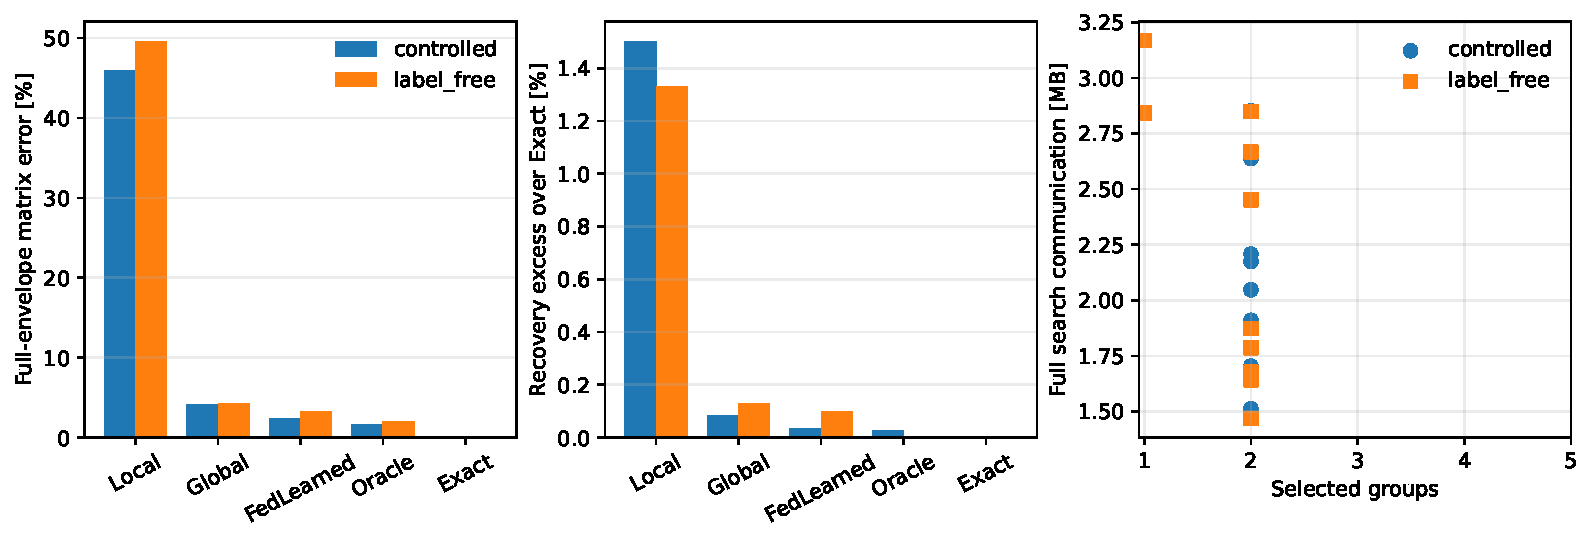
\includegraphics[width=0.98\linewidth]{../results/figures/experiment_10e_federated_latent_groups.pdf}
\caption{Experiment 10E identification, control, and full-search communication
results for controlled and label-free coverage.}
\label{fig:experiment10e}
\end{figure}

\paragraph{Federated-equivalence result.}
The gate passes in all 20 fleet--coverage conditions. Federated and centralized
latent grouping select identical partitions and group counts. The maximum
coefficient difference is $3.20\times10^{-14}$ and the maximum BIC difference
is $1.87\times10^{-9}$. CentralLearned and FederatedLearned consequently have
identical reported prediction and control metrics. The result verifies the
distributed sufficient-statistic implementation rather than merely assuming
that centralized clustering transfers to FL.

\paragraph{Label-free sharing result.}
Removing family-stratified coverage weakens but does not remove the benefit.
FederatedLearned reduces matrix error by 93.41\% and recovery by 1.216\%
relative to Local, with positive intervals and ten wins. Against Global it
reduces matrix error by 23.74\%. The recovery improvement over Global is only
0.031\%, despite its positive interval, and is too small to carry a practical
control-superiority claim.

The label-free protocol also exposes why compatibility should not be equated
with physical family. In seed 375, no nominal-family client observes the final
28--30~m/s block. OracleFamily therefore lacks the required scheduling
coverage and produces an infeasible 30~m/s controller, whereas
FederatedLearned remains feasible. Learned compatibility accounts jointly for
dynamics and information coverage; a correct physical label alone does not
guarantee an identifiable group model.

\paragraph{Selected groups and communication.}
Controlled coverage selects two groups in all ten fleets. Label-free coverage
selects two groups in eight fleets and a single group in two, with mean ARI
0.352. The full candidate search requires on average 45.0 model/assignment
rounds and 2.04~MB per controlled fleet, or 48.9 rounds and 2.24~MB per
label-free fleet, assuming 64-bit scalars. These totals include every restart
and every candidate $K$, not only the final selected model. The absolute load
is modest, but the exhaustive multistart search is not communication efficient
and should not be advertised as such.

\paragraph{Decision.}
Experiment 10E establishes the missing genuine-FL component: locally retained
data, additive client updates, iterative label-free group assignment, unknown
group count, and explicit end-to-end communication accounting. It also confirms
that complementary sharing remains beneficial without family-aware coverage.
It does not resolve the principal control-story weakness. FederatedLearned and
Global remain almost indistinguishable under the recovery test. The next
experiment must therefore use speed-varying tracking, steering constraints,
and worst-client metrics to determine whether the substantially better learned
LPV models provide a practically meaningful control advantage.

\paragraph{Reproducibility.}
The configuration and implementation are in
\path{code/config/experiment_10e.json} and
\path{code/experiments/experiment_10e_federated_latent_groups.py}. Per-fleet
records, assignments, candidate scores, communication counts, aggregate
summaries, paired intervals, and provenance hashes are stored under
\path{results/tables}.
